\documentclass[12pt,reqno]{amsart}
%\documentclass[../Solutions_Introduction_to_Algorithms.tex]{subfiles}
\usepackage{amsmath,amsfonts,amscd,amssymb,epsf,color,enumerate,graphicx,url}
\usepackage{algorithm, algorithmic}
\usepackage{forest, tikz, xcolor}
\usepackage{parskip}
\usetikzlibrary{matrix, positioning}
\usetikzlibrary{positioning,arrows.meta}
\setlength{\oddsidemargin}{-0.2in}%
\setlength{\evensidemargin}{-0.2in}%
\setlength{\textwidth}{6.6in}%
\setlength{\topmargin}{-0.5in}%
 \setlength{\textheight}{9.5in}%
 \definecolor{orange}{rgb}{1,0.5,0}
 \pagestyle{plain}
\linespread{1.3}
\usepackage[small]{caption}
\newcommand{\pa}{\partial}
\newcommand{\va}{\vspace{0.4cm}}
\newcommand{\di}{\displaystyle}
\newcommand{\disp}{\displaystyle}


% turn on \answertrue to show the solution
% turn on \answerfalse to hide the solution
\newif\ifanswer
\answertrue
%\answerfalse



\begin{document}
\noindent {\footnotesize Introduction to Algorithms}\hspace{10.5cm} {\footnotesize Solutions}

\vspace{0.5cm}
\hspace{5.5cm}\textbf{\large Exercises in Section 2.1}
\vspace{0.5cm}

\begin{enumerate}[1.]

\item Using Figure~2.2 as a model, illustrate the operation of \textsc{Insertion-Sort} on an array initially containing the sequence $\langle 31, 41, 59, 26, 41, 58 \rangle$.
\vspace{0.5cm}

\ifanswer
\noindent {\bf Solution}

\begin{center}
    \begin{tikzpicture}[>=Stealth,scale=1]

    \fill[orange!25] (1,0) rectangle ++(1,1);
    \fill[blue!25] (2,0) rectangle ++(1,1);

    \foreach \i/\v in {1/31,2/41,3/59,4/26,5/41,6/58}{
    \draw (\i,0) rectangle ++(1,1);
    \node at (\i+0.5,0.5) {\v};
    \node[above] at (\i+0.5,1) {\small \i};
    }

    \draw[->,blue,thick,bend left=60] (2.9,0) to (2.1,0);

    \node[left] at (0.7,0.5) {(a)};
    \end{tikzpicture}\\
    \vspace{0.5cm}


    \begin{tikzpicture}[>=Stealth,scale=1]

    \fill[orange!25] (1,0) rectangle ++(1,1);
    \fill[orange!25] (2,0) rectangle ++(1,1);
    \fill[blue!25] (3,0) rectangle ++(1,1);

    \foreach \i/\v in {1/31,2/41,3/59,4/26,5/41,6/58}{
    \draw (\i,0) rectangle ++(1,1);
    \node at (\i+0.5,0.5) {\v};
    \node[above] at (\i+0.5,1) {\small \i};
    }

    \draw[->,blue,thick,bend left=60] (3.9,0) to (3.1,0);

    \node[left] at (0.7,0.5) {(b)};
    \end{tikzpicture}\\
    \vspace{0.5cm}


    \begin{tikzpicture}[>=Stealth,scale=1]

    \fill[orange!25] (1,0) rectangle ++(1,1);
    \fill[orange!25] (2,0) rectangle ++(1,1);
    \fill[orange!25] (3,0) rectangle ++(1,1);
    \fill[blue!25] (4,0) rectangle ++(1,1);

    \foreach \i/\v in {1/31,2/41,3/59,4/26,5/41,6/58}{
    \draw (\i,0) rectangle ++(1,1);
    \node at (\i+0.5,0.5) {\v};
    \node[above] at (\i+0.5,1) {\small \i};
    }

    \draw[->,orange,thick,bend left=40] (1.5,0) to (2.5,0);
    \draw[->,orange,thick,bend left=40] (2.5,0) to (3.5,0);
    \draw[->,orange,thick,bend left=40] (3.5,0) to (4.5,0);
    \draw[->,blue,thick,bend left=40] (4.8,0) to (1.2,0);

    \node[left] at (0.7,0.5) {(c)};
    \end{tikzpicture}\\
    \vspace{0cm}


    \begin{tikzpicture}[>=Stealth,scale=1]

    \fill[orange!25] (1,0) rectangle ++(1,1);
    \fill[orange!25] (2,0) rectangle ++(1,1);
    \fill[orange!25] (3,0) rectangle ++(1,1);
    \fill[orange!25] (4,0) rectangle ++(1,1);
    \fill[blue!25] (5,0) rectangle ++(1,1);

    \foreach \i/\v in {1/26,2/31,3/41,4/59,5/41,6/58}{
    \draw (\i,0) rectangle ++(1,1);
    \node at (\i+0.5,0.5) {\v};
    \node[above] at (\i+0.5,1) {\small \i};
    }

    \draw[->,orange,thick,bend left=40] (4.5,0) to (5.5,0);
    \draw[->,blue,thick,bend left=40] (5.8,0) to (4.2,0);

    \node[left] at (0.7,0.5) {(d)};
    \end{tikzpicture}\\
    \vspace{0.5cm}


    \begin{tikzpicture}[>=Stealth,scale=1]

    \fill[orange!25] (1,0) rectangle ++(1,1);
    \fill[orange!25] (2,0) rectangle ++(1,1);
    \fill[orange!25] (3,0) rectangle ++(1,1);
    \fill[orange!25] (4,0) rectangle ++(1,1);
    \fill[orange!25] (5,0) rectangle ++(1,1);
    \fill[blue!25] (6,0) rectangle ++(1,1);

    \foreach \i/\v in {1/26,2/31,3/41,4/41,5/59,6/58}{
    \draw (\i,0) rectangle ++(1,1);
    \node at (\i+0.5,0.5) {\v};
    \node[above] at (\i+0.5,1) {\small \i};
    }

    \draw[->,orange,thick,bend left=40] (5.5,0) to (6.5,0);
    \draw[->,blue,thick,bend left=40] (6.8,0) to (5.2,0);

    \node[left] at (0.7,0.5) {(e)};
    \end{tikzpicture}\\
    \vspace{0.5cm}


    \begin{tikzpicture}[>=Stealth,scale=1]

    \fill[orange!25] (1,0) rectangle ++(1,1);
    \fill[orange!25] (2,0) rectangle ++(1,1);
    \fill[orange!25] (3,0) rectangle ++(1,1);
    \fill[orange!25] (4,0) rectangle ++(1,1);
    \fill[orange!25] (5,0) rectangle ++(1,1);
    \fill[orange!25] (6,0) rectangle ++(1,1);

    \foreach \i/\v in {1/26,2/31,3/41,4/41,5/58,6/59}{
    \draw (\i,0) rectangle ++(1,1);
    \node at (\i+0.5,0.5) {\v};
    \node[above] at (\i+0.5,1) {\small \i};
    }

    \node[left] at (0.7,0.5) {(f)};
    \end{tikzpicture}\\
    \vspace{0.5cm}
\end{center}

\vspace{1cm}



\item Consider the procedure \textsc{Sum-Array} on the facing page. It computes the sum of the $n$ numbers in array $A[1\!:\!n]$. State a loop invariant for this procedure, and use its initialization, maintenance, and termination properties to show that the \textsc{Sum-Array} procedure returns the sum of the numbers in $A[1\!:\!n]$.

\begin{algorithm}
    \caption{\textsc{Sum-Array}$(A, n)$}
    \begin{algorithmic}[1]
        \STATE $sum = 0$
        \FOR{$i = 1$ to $n$}
            \STATE $sum = sum + A[i]$
        \ENDFOR
        \RETURN $sum$
    \end{algorithmic}
\end{algorithm}

\vspace{0.5cm}

\ifanswer
\noindent {\bf Solution}

\textbf{Loop invariant:} At the start of each iteration, $sum$ is equal to the sum of the first $i$ numbers in $A$.\\
\textbf{Initialization:} Before the first iteration, $sum = 0$.\\
\textbf{Maintenance:} Suppose that at the start of the $i$-th iteration, $sum = \sum_{j=1}^{i-1} A[j]$. Then at the start of the $(i+1)$-th iteration, $sum = \sum_{j=1}^{i} A[j]$.\\
\textbf{Termination:} When $i = n$, the loop terminates. Then $sum = \sum_{j=1}^{n} A[j]$.\\

\vspace{1cm}



\item Rewrite the \textsc{Insertion-Sort} procedure to sort into monotonically decreasing instead of monotonically increasing order.
\vspace{0.5cm}

\ifanswer
\noindent {\bf Solution}

\begin{algorithm}
    \caption{\textsc{Insertion-Sort}$(A, n)$}
    \begin{algorithmic}[1]
        \FOR{$i = 2$ to $n$}
            \STATE $key = A[i]$
            \STATE $j = i - 1$
            \WHILE{$j > 0$ and $A[j] < key$}
                \STATE $A[j+1] = A[j]$
                \STATE $j = j - 1$
            \ENDWHILE
            \STATE $A[j+1] = key$
        \ENDFOR
    \end{algorithmic}
\end{algorithm}

\vspace{1cm}



\item Consider the \emph{searching problem}: \textbf{Input:} A sequence of $n$ numbers $\langle a_1, a_2, \ldots, a_n\rangle$ stored in array $A[1\!:\!n]$ and a value $x$. \textbf{Output:} An index $i$ such that $x = A[i]$, or the special value \textsc{nil} if $x$ does not appear in $A$. Write pseudocode for \emph{linear search}, which scans through the array from beginning to end, looking for $x$. Using a loop invariant, prove that your algorithm is correct. Make sure that your loop invariant fulfills the three necessary properties.
\vspace{0.5cm}

\ifanswer
\noindent {\bf Solution}

\begin{algorithm}
    \caption{\textsc{Linear-Search}$(A, n, x)$}
    \begin{algorithmic}[1]
        \FOR{$i = 1$ to $n$}
            \IF{$A[i] = x$}
                \RETURN $x$
            \ENDIF
        \ENDFOR
        \RETURN $NIL$
    \end{algorithmic}
\end{algorithm}\vspace{1cm}



\item Consider the problem of adding two $n$-bit binary integers $a$ and $b$, stored in two
$n$-element arrays $A[0\!:\!n-1]$ and $B[0\!:\!n-1]$, where each element is either $0$
or $1$, $a = \sum_{i=0}^{n-1} A[i]\cdot 2^{i}$ and $b = \sum_{i=0}^{n-1} B[i]\cdot 2^{i}$.
The sum $c = a + b$ of the two integers should be stored in binary form in an
$(n+1)$-element array $C[0\!:\!n]$, where $c = \sum_{i=0}^{n} C[i]\cdot 2^{i}$.
Write a procedure \textsc{Add-Binary-Integers} that takes as input arrays $A$ and $B$,
along with the length $n$, and returns array $C$ holding the sum.

\vspace{0.5cm}

\ifanswer
\noindent {\bf Solution}

\begin{algorithm}
    \caption{\textsc{Add-Binary-Integers}$(A, B, C, n)$}
    \begin{algorithmic}[1]
        \STATE Initialize $C$ with all zeros.
        \FOR{$i = 0$ to $n - 1$}
        \STATE $C[i] = A[i] + B[i] + C[i]$
            \IF{$C[i] > 1$}
                \STATE $C[i + 1] = 1$
                \STATE $C[i] = C[i] - 2$
            \ENDIF
        \ENDFOR
        \RETURN $NIL$
    \end{algorithmic}
\end{algorithm}\vspace{1cm}





\end{enumerate}

\end{document}



